% !TeX root = ../main.tex
% Add the above to each chapter to make compiling the PDF easier in some editors.

\chapter{Related Work}\label{chapter:relatedwork}
\section{Risks}
While working with sensitive data, we have to assess multiple attack vectors before we can take action. We compile possible attack vectors and how they could be solved.

\subsection{Risks of centralization}
Because of efficiency, centralized information systems have always been a go-to infrastructure. The advantages of simple deployment, ease of maintenance, and less bureaucracy will always be an incentive for big companies and governments to consider it. In 1965, the US Social Science Research Council \cite{lawreview} proposed a National Data Center to store all data in a central location for statistical data analysis. Still, in the end, the plans for the system were shot down because of the lack of privacy protection.

Today, many big tech companies are collecting data about their users and storing them in central databases. Nevertheless, centralization has a fatal flaw in protecting privacy. According to Stolpe \cite{DBLP:journals/sigkdd/Stolpe16}, the collection of sensitive data in one location poses a high risk to their originator.

Centralized databases that store private information are one of the weak points that have been under constant attack for years. After an analysis by RiskBased Security \cite{riskbasedsecurity}, they determined that in the first three quarters of 2019, there have been over 5000 data breaches, with almost 8 billion records exposed, 33\% more compared to the number reported in the first nine months of the previous year. Around 10\% of those breaches originated from the inside, such as accidental leaks and intentional publications.

The vulnerability of central databases makes private data stored prone to attacks from inside, as well as outside.

\subsection{Reconstruction, linkage and tracing attacks}
The first reaction to those data breaches would naturally be to de-identify the data. If we do that by stripping away all sensitive information, making the data set pseudonymous, the risk of private data leaking remains, which can be exploited by reconstruction, linkage, and tracing attacks. The most severe problem is the danger of re-identification \cite{reidentification}\cite{DBLP:journals/midm/EmamBTNJV11}\cite{DBLP:journals/midm/DankarENR12}.
It enables adversaries to deduce the identity of an individual using other publicly available data sets or auxiliary knowledge. 
In her work, Sweeney \cite{DBLP:journals/ijufks/Sweene02} was able to re-identify former Massachusetts governor William Weld by linking medical records from the Group Insurance Commission and the voter registration list.

The goal of reconstruction is to determine sensitive data from a data set that has been generalized or suppressed using publicly available information \cite{DBLP:journals/fttcs/DworkR14}\cite{exposed}. Lacharite\'e \cite{DBLP:conf/sp/LachariteMP18} has proven that efficient reconstruction attacks are very well possible, given a dense data set.
 
Tracing, on the other hand, is the ability to identify if an individual is present in a data set or not \cite{exposed}. It can expose information, which has previously been unknown. Homer et al. \cite{dna} showed how they were able to determine the presence or absence of a target in their genome-wide association study.

\subsection{Risks of location tracking}
In regards to location data, the ability to infer the home and work location poses both risks for privacy and life and limb. Research \cite{DBLP:conf/pervasive/Krumm07}\cite{DBLP:journals/corr/abs-1901-00897}\cite{DBLP:conf/pervasive/GolleP09} has shown that it is possible to track individuals, deduce their home address and even their workplace using historical location data.
Location data is also able to hold more information than just spatial and temporal data. It is possible to associate a spatial location with other sensitive information. For example, the attendance of a political rally can tell an adversary about the political affiliation, or tracking someone to a specialized clinic could expose additional medical data.
Besides, being able to analyze the movement pattern and predict the presence of people in a particular location may put their lives in danger. Being able to determine the presence of people in their homes or their absence might enable someone to break in and rob their house.

\section{Countermeasures}
To implement a secure platform that is less vulnerable to the problems proposed in the sections above, we look into methods and design decisions to prevent them.
\subsection{Distribution and decentralization}
When the Advanced Research Projects Agency Network (ARPANET) implemented the prototype of the internet in 1969, it was a decentralized network of computers scattered across the United States. With the adoption of the TCP/IP in 1982, it became the internet, an interconnected network of networks as we have today \cite{DBLP:books/daglib/0006297}.
In 1989, Tim Berners-Lee introduced the world wide web as a read-only means of accessing information from other computers, and the commercialization turned it into the centralized web we know today. 

The dangers of data breaches can originate from outside the companies as well as inside, and their cause range from poorly implemented security and lax security policies to human error \cite{riskbasedsecurity}.
Figure \ref{fig:comparison} depicts two alternatives in place of a centralized architecture: distributed and decentralized.

\begin{figure}[htpb]
  \centering
  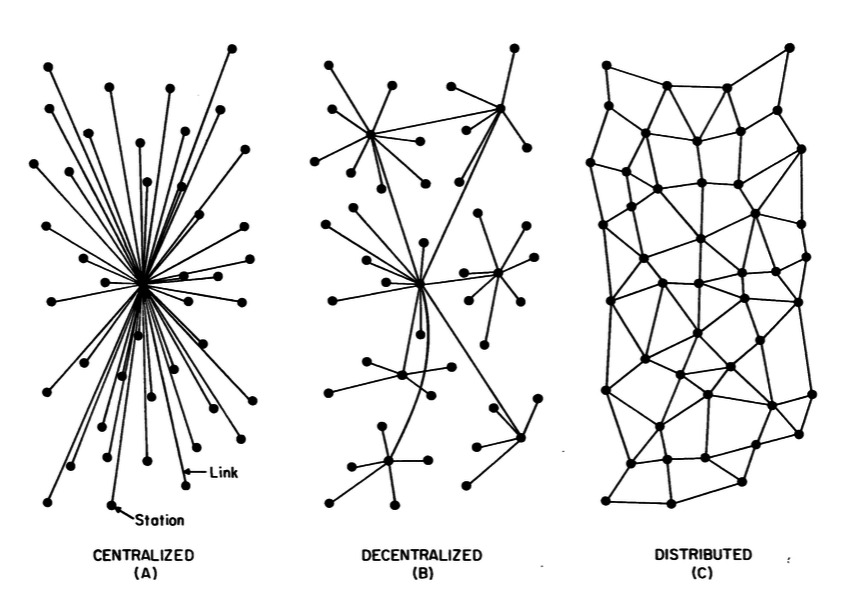
\includegraphics[width=0.8\textwidth]{figures/comparison.jpg}
  \caption{Illustration of a centralized, distributed and decentralized architecture \cite{distributed}} 
  \label{fig:comparison}
\end{figure}

In the last decade, we have seen a rise in attempts to reorganize the internet. This trend amassed attention in 2009 when the creator under the pseudonym Satoshi Nakamoto  \cite{bitcoin} created Bitcoin, "A Peer-to-Peer Electronic Cash System" leveraging blockchain technology, followed by the Ethereum \cite{ethereum} platform in 2013.
The goal of decentralization is the separation of power from a single instance. In our case, it would be to take away control from monopolies over our data. 

One of the protocols that arose from this niche is the InterPlanetary File System (IPFS)\cite{DBLP:journals/corr/Benet14}. IPFS is a peer-to-peer hypermedia protocol to make the web more decentralized and distributed. A node can upload a file, and every file and its blocks generate a cryptographic hash, making it content addressable. Requesting a file will search the network for nodes that store it, and the nodes that have it will provide.

Distribution takes decentralization a step further by eliminating the central control by giving all instances the same amount of power. Using distributed storage, in place of a centralized database, removes the single point of vulnerability and lowers the effort-to-reward balance and thus might deter malicious actors from trying to steal data.

\subsection{Homomorphic encryption}
Conventionally, encryption methods do not provide anonymity. However, one could argue that, in a way, anonymity is provided when the data is not readable or accessible. If an adversary manages to steal a data set while it is still encrypted, they will not be able to infer identity or any additional information, unless they are able to decrypt it beforehand. 

Homomorphic encryption enables the arithmetic operations on an encrypted data set. They are separated into three categories \cite{DBLP:journals/corr/abs-1812-02428}:
\begin{itemize}
    \item \textbf{Fully Homomorphic Encryption (FHE)} allows multiple arbitrary operations, but has a lot of overhead and thus is computationally expensive.
    \item \textbf{Somewhat Homomorphic Encryption (SWHE)} supports only selected operations to a limited number of times and is computationally more feasible.
    \item \textbf{Partially Homomorphic Encryption (PHE)} enables one type of operation any number of times.
\end{itemize}

It protects the data set from intermediate parties, making them unable to derive private data, while still making it possible to work on it. We will look into possible implementations and figure out if this encryption scheme is feasible in a mobile environment.

\subsection{k-Anonymity}
Sweeney \cite{DBLP:journals/ijufks/Sweene02} has shown that anonymous data sets are not as anonymous as they seem. Quasi-identifiers, an identifier or a combination of non-identifying attributes, still enable malicious actors to link individuals back to their data. As one of the possible countermeasures to this problem, she proposes k-anonymity. This is achieved when every query for quasi-identifier returns at least k results. A quasi-identifier, such as ZIP code, birth date, or sex, can be used to link with external data sources to create new identifiers. For this, Samarati \cite{samarati} and Sweeney \cite{DBLP:journals/ijufks/Sweene02} suggest the use of generalization and suppression.

Former is realized by expanding specific attributes into ranges. For instance, instead of assigning the real age, an age range is substituted, resulting in a loss of accuracy, but a higher degree of anonymity. For the latter, there are two methods of suppression. Attribute suppression removes attributes from the data set, reducing the number of possible quasi-identifiers by lowering the number of possible combinations. In contrast, record suppression, on the other hand, deletes entire entries in the data set to take out unique entries that do not meet the criteria of k-anonymity \cite{singapore}.

\subsection{Differential privacy}
In 2006, Dwork \cite{DBLP:conf/icalp/Dwork06} proposed a mathematical definition for differential privacy. It is used to prevent statistical databases from leaking private information. It is a compelling definition that is able to guarantee privacy. An algorithm is differential private as long as it prevents tracing attacks, meaning that output does not show signs of a particular individual is present in it or not. Removing an entry in the data set would not reflect in the resulting queries.
Both Google \cite{erlingsson_2014} and Apple \cite{apple} have implemented differential privacy into their data collection methods.

Differential privacy guarantees three qualities:
\begin{itemize}
    \item All data about an individual in the database is protected even if the adversary manages to learn auxiliary information about all other entries in the data set.
    \item Two differently differential private data sets can be combined, and the resulting data set is still differential private.
    \item It is possible to quantify the loss of privacy and information gained by the malicious actor.
    \item It can be applied to groups.
\end{itemize}

Noise is added to the data to achieve differential privacy,  but replay attacks might be able to reveal actual values. To avoid this, the default noise function used is the Laplacian mechanism or exponential mechanism \cite{DBLP:journals/fttcs/DworkR14}. The noise function also has to be modified to the extent of the sensitivity of the data set. That is the maximum value a single entry in the data set can change the query. For example, a query for the count of true and false answers; the sensitivity is one as the removal of one participant only removes one response of true or false. Nevertheless, the higher the sensitivity, the greater the noise that has to be added to the data to guarantee privacy, which in subsequently makes the data less accurate. The noise can be added either on the aggregation of the user data or on the aggregated data itself.

\subsubsection{Global Differential Privacy}
If the noise function is applied to the entire aggregated raw data set, it is called global differential privacy. It works by using a noise function on the result of a query, as depicted in Figure \ref{fig:global_diff}. The advantage of this model is that the resulting data set is still very accurate, but on the downside, the whole raw data set has to be available to use this function.

\begin{figure}[htpb]
  \centering
  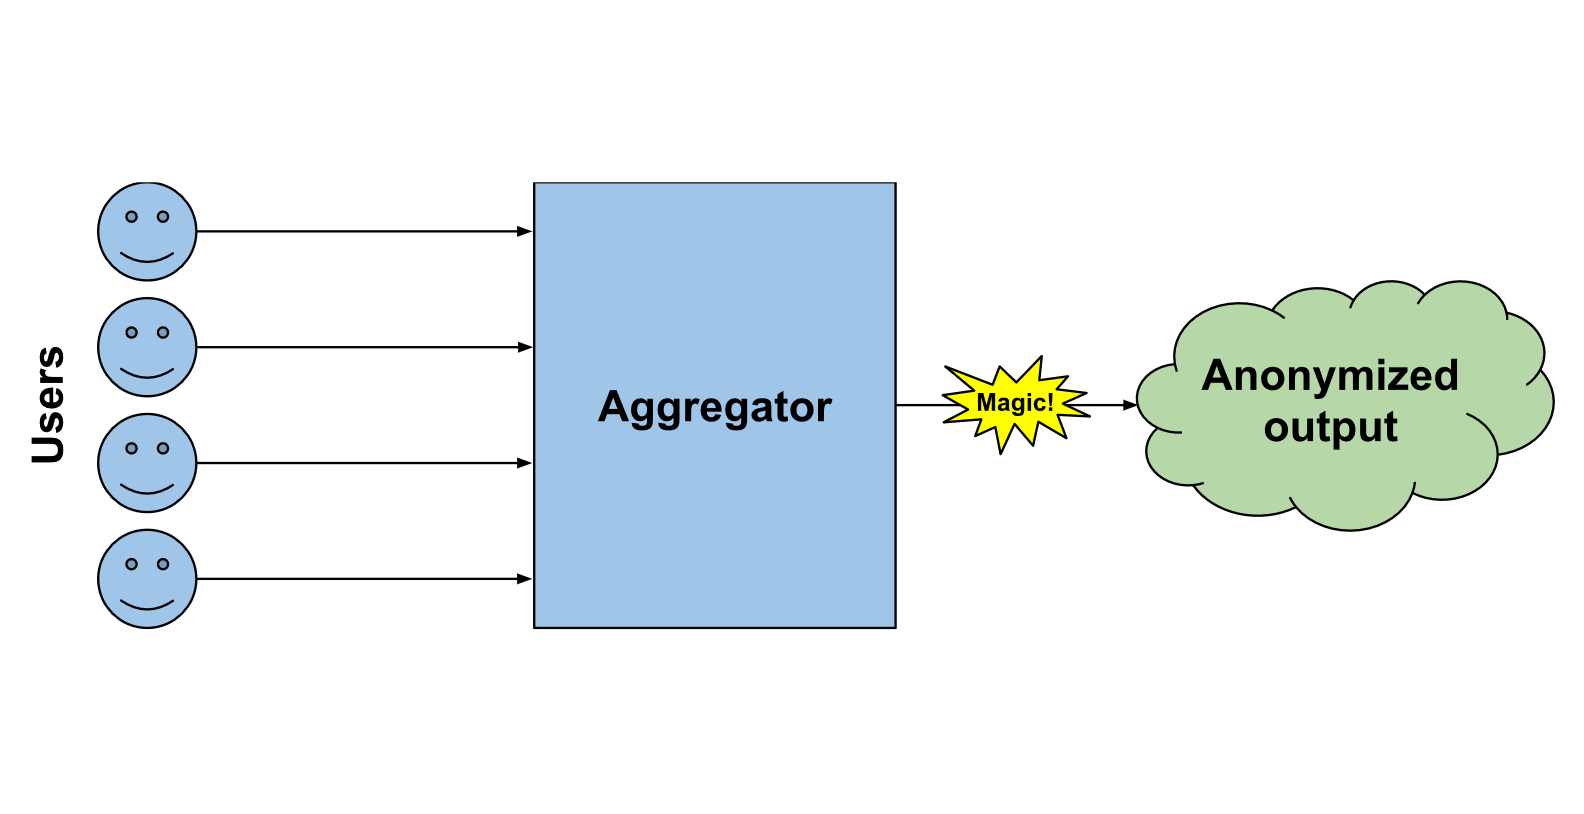
\includegraphics[width=0.8\textwidth]{figures/global_diff.png}
  \caption{Illustration of a global differential data flow\cite{desfontaines}}
  \label{fig:global_diff}
\end{figure}

\subsubsection{Local Differential Privacy}
Figure \ref{fig:local_diff} shows that differential privacy can also be used on each entry of the data. By running every entry through the mechanism, it creates a locally differential private data set. The disadvantage of this method is the much higher noise, but in exchange, the raw data itself is protected and does not require trust to an intermediate aggregator.

\begin{figure}[htpb]
  \centering
  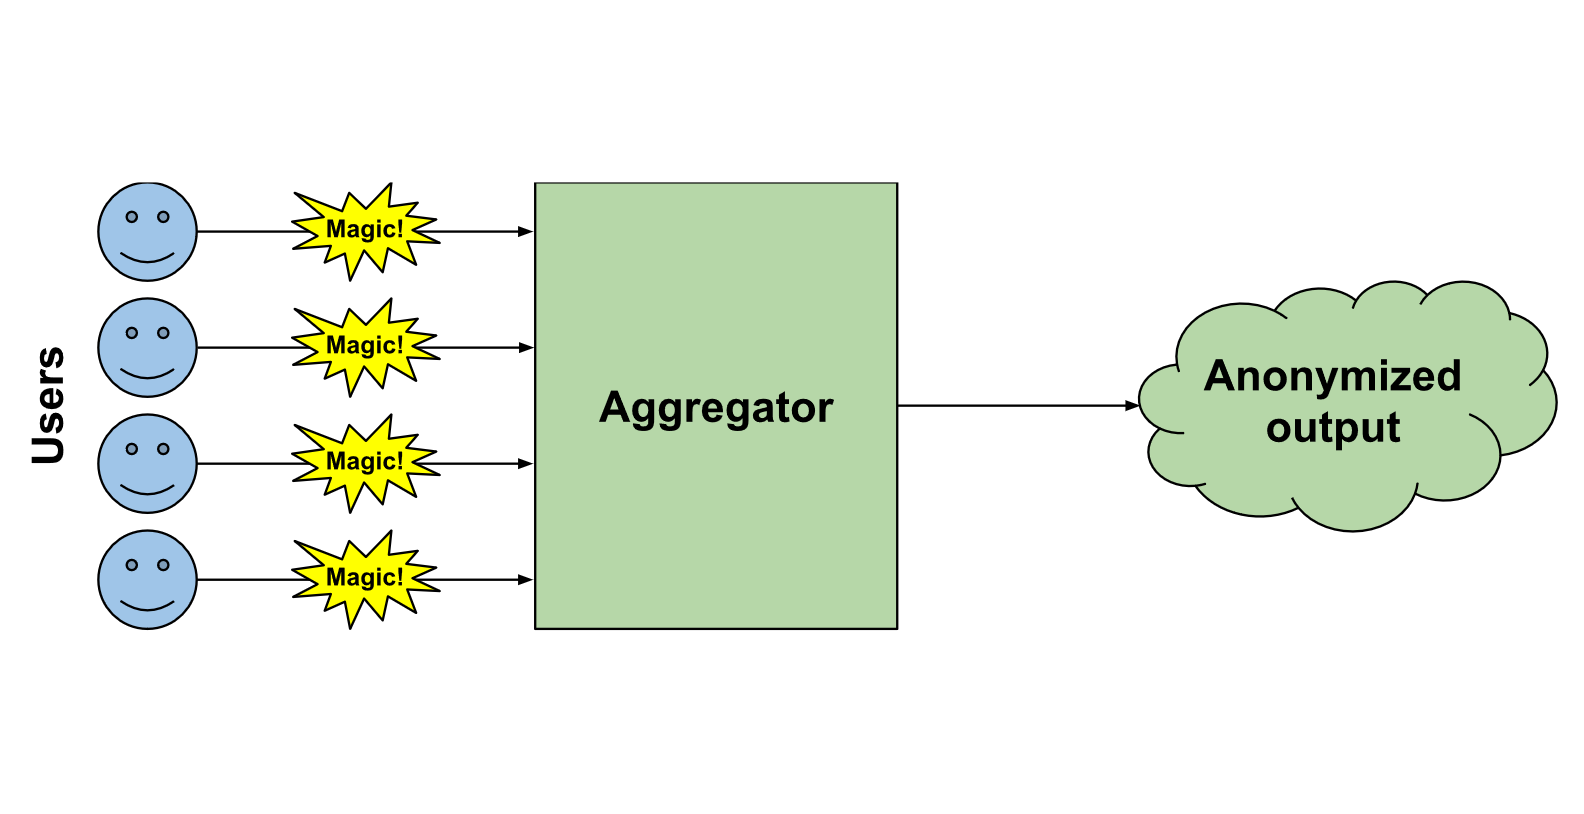
\includegraphics[width=0.8\textwidth]{figures/local_diff.png}
  \caption{Illustration of a local differential data flow \cite{desfontaines}} 
  \label{fig:local_diff}
\end{figure}

A typical example of this is the coin toss. A survey asks a question that can be answered with a yes or no. The function would toss a coin and would answer the question honestly on heads and otherwise answer the question with a second coin toss, with heads resulting in yes and tails in no. 

\subsection{Spatial Cloaking}
As mentioned above, spatial data can reveal a lot of sensitive information about a person. So location privacy should always be a high priority. Many algorithms can be used to hide the real location in a general area.

\subsubsection{Casper}
Casper \cite{DBLP:journals/tods/ChowMA09} is a grid-based cloaking mechanism that organizes the location in squares and structures the level of detail like a pyramid. It cloaks the real coordinates by using the lower-left corner and upper-right corners as a designated area of the location \cite{DBLP:conf/ssd/TanLM09}. The Figure \ref{fig:casper} would show the lowest level of detail with \(\langle(0,0),(4,4)\rangle\), covering the whole area, and the highest level of detail with \(\langle(0,2),(1,3)\rangle\), only wrapping a small portion of the area. The algorithm looks for neighboring areas for other users and then spans the whole area when it finds one to fulfill the requirements of k-anonymity. For example, \(U_1\) with its cloaked area \(\langle(0,2),(1,3)\rangle\) would need the area \(\langle(1,2),(2,3)\rangle\) to satisfy \(k=4\).

\begin{figure}[htpb]
  \centering
  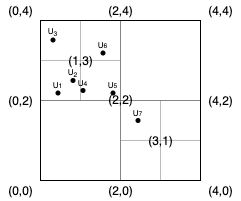
\includegraphics[width=0.5\textwidth]{figures/casper.png}
  \caption{Illustration of spatially cloaked squared areas} 
  \label{fig:casper}
\end{figure}

\subsubsection{Interval Cloaking}
Similarly to Casper, Interval Cloaking also uses rectangular cloaking areas to hide the real locations. However, instead of using neighboring squares, it uses a lower level of detail to achieve k-anonymity. Using the example from above, Interval Cloaking would span the anonymized spatial area over \(\langle(0,2),(2,4)\rangle\) to assure k-anonymity with \(k=4\) for \(U_1\) \cite{DBLP:conf/ssd/TanLM09}\cite{DBLP:conf/pet/ChengZBP06}.

\subsubsection{Hilbert Cloaking}
Another famous spatial cloaking algorithm is Hilbert Cloaking \cite{DBLP:conf/socialcom/UmKC10}. It uses the Hilbert space-filling curve to map the 2-dimensional area into a 1-dimensional representation. Then it groups together points depending on the provided \(k\) because points that are in proximity on the Hilbert curve are also close to each other in 2D. Instead of using predetermined rasterization of the area, the cloaked area is spanned by the users themselves \cite{DBLP:journals/is/GhinitaZPK10}\cite{DBLP:journals/sigkdd/Gkoulalas-DivanisKV10},\cite{DBLP:conf/ssd/TanLM09}.
